\section{Stronger baselines and available requests}
\subsection{Follow-up design}
The initial heuristic alone cannot establish whether profile-guided placement is useful. We therefore add the published RCM, Gorder and Porder routines of Coleman et al.~\cite{coleman}. RCM reverses a degree-ordered Cuthill--McKee traversal \cite{cuthill}. Gorder \cite{gorder} scores graph relationships to a recent placement window; Porder weights them using query traversal frequencies. Both use the supplied five-node window. Porder assigns one plus the training traversal count to each base-layer edge. The local query-aware method instead weights co-visited pairs and uses footprint-specific block grouping.

The adapter applies the supplied permutations to the separate vector array and preserves the source's window-expiration condition. An ordered-set helper replaces the weighted linked-list queue with matching score and tie semantics. All three methods match the untouched reference on 30 weighted graphs, and sanitizer runs preserve the normal mappings on the full graph. This evaluates their placement routines under a different memory representation; it does not reproduce the authors' cache-aware application benchmark.

To test available work, the follow-up drains an adjacency payload before offering its candidate vectors, then drains those vectors before the next expansion. Entry reads receive separate phases. Candidate membership is checked against the preceding list. Figure~\ref{fig:phases} illustrates this memory-boundary model. It permits overlap among a phase's candidates under the same 64-transaction bound, without executing distance computation. A phase-to-query map reconstructs original-query service including inter-phase gaps.

\begin{figure*}[t]\centering
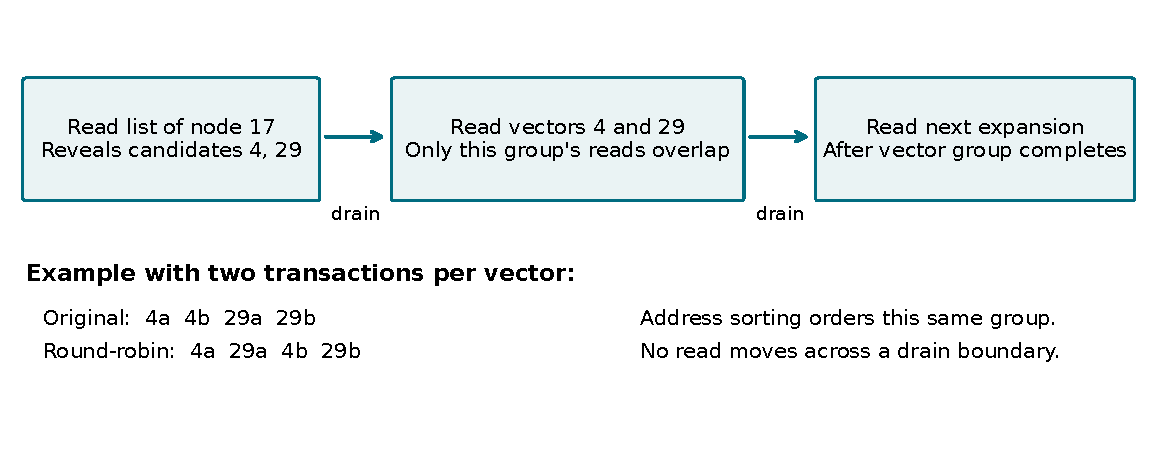
\includegraphics[width=0.92\textwidth]{generated/followup_phases.pdf}
\caption{Expansion-bounded replay. Only transactions within the candidate-vector group are reordered. The illustration uses two chunks per vector; the experiment uses sixteen at 512 bytes and four at 128 bytes. Drain boundaries wait for completions while retaining row state.}\label{fig:phases}
\end{figure*}

Address sorting and transaction round-robin use only a phase's available reads. The former orders their addresses; the latter sends the first chunk of every vector, then the second, and so on. Every duplicate transaction remains present, and none crosses a phase. Scheduling and buffering overhead are omitted. This is a defined dependency sensitivity, not instruction-level HNSW or an integrated PIM engine.

The fixed matrix adds 494 replays on all 19 graph/split pairs and both widths: three new flat placements, six bounded placements, and two schedules on BFS and query-aware placement. Four further command-recording repeats diagnose the pilot's scheduling contrast without changing its timings. All 791 earlier results remain available. These extensions reuse previously evaluated queries and remain exploratory.

\subsection{What placement and ordering change}
Table~\ref{tab:published} compares published layouts against BFS with matching expansion boundaries. The full thesis retains all six placements against identity and BFS, under both flat and bounded replay. This prevents a result from the local heuristic from standing in for the whole class of trained layouts.

\begin{table}[htbp]\centering\small
\caption{Published placement routines under bounded replay. Mean cycle differences and 95\% intervals over ten reference splits. Negative means fewer cycles than matching BFS.}\label{tab:published}
\begin{tabular}{lrr}
\toprule
Bytes & Layout & $\Delta$ vs. BFS (\%) \\
\midrule
512 & RCM & -0.16 [-0.21, -0.11] \\
512 & Gorder & -0.20 [-0.24, -0.16] \\
512 & Porder & -0.38 [-0.47, -0.28] \\
128 & RCM & -0.47 [-0.55, -0.38] \\
128 & Gorder & -1.33 [-1.42, -1.25] \\
128 & Porder & -1.19 [-1.33, -1.04] \\
\bottomrule
\end{tabular}

\end{table}

Figure~\ref{fig:schedules} shows the size and sign of the scheduling effects. Table~\ref{tab:schedules} reports comparisons that change only order within matching BFS phases. At 512 bytes, the round-robin mean saving is \RoundRobinBFSSavedFloat{} controller cycles per original query. Across the 19 graph/split cases, \RRFasterQueriesFloat\% of query records improve in each case. The empirical 95th-percentile service differences range from \RRPtailRangeFloat\%. These are descriptive within-case checks, not independent replications or application latency guarantees. The round-robin sign persists across the selected constructions on both evaluated placements. Placement itself is less uniform: expansion boundaries reverse a small query-aware 512-byte advantage on graph seed 101, split two. Construction-specific ranges and all scheduling results are retained in the thesis and artifact.

\begin{table}[htbp]\centering\small
\caption{Available-request schedules on BFS. Mean cycle differences and 95\% intervals over ten reference splits, relative to original-order bounded replay. The smaller footprint remains hypothetical.}\label{tab:schedules}
\begin{tabular}{lrr}
\toprule
Bytes & Schedule & $\Delta$ vs. original (\%) \\
\midrule
512 & Sorted & +0.19 [+0.13, +0.24] \\
512 & Round-robin & -14.58 [-14.64, -14.51] \\
128 & Sorted & +0.17 [+0.12, +0.21] \\
128 & Round-robin & +3.43 [+3.31, +3.55] \\
\bottomrule
\end{tabular}

\end{table}

The first split's command accounting explains the contrasting widths. At 512 bytes, round-robin adds \RRCmdExtraFloat{} command cycles but removes \RRNoCmdDeltaFloat{} no-command cycles, saving \RRStreamDeltaFloat{} overall. Offered bank diversity within complete 64-request phase windows grows from \RRBanksBeforeFloat{} to \RRBanksAfterFloat{}, despite a lower row-hit fraction. At 128 bytes, extra row operations and no-command cycles together cost \RRStreamDeltaCompact{} cycles. Its original stream already exposes more vectors through the transaction bound. The accounting supports the role of bank exposure and row reuse; it does not isolate every timing restriction. Even mean read latency falls in both cases, showing why completed-work timing remains necessary.

\begin{figure*}[t]\centering
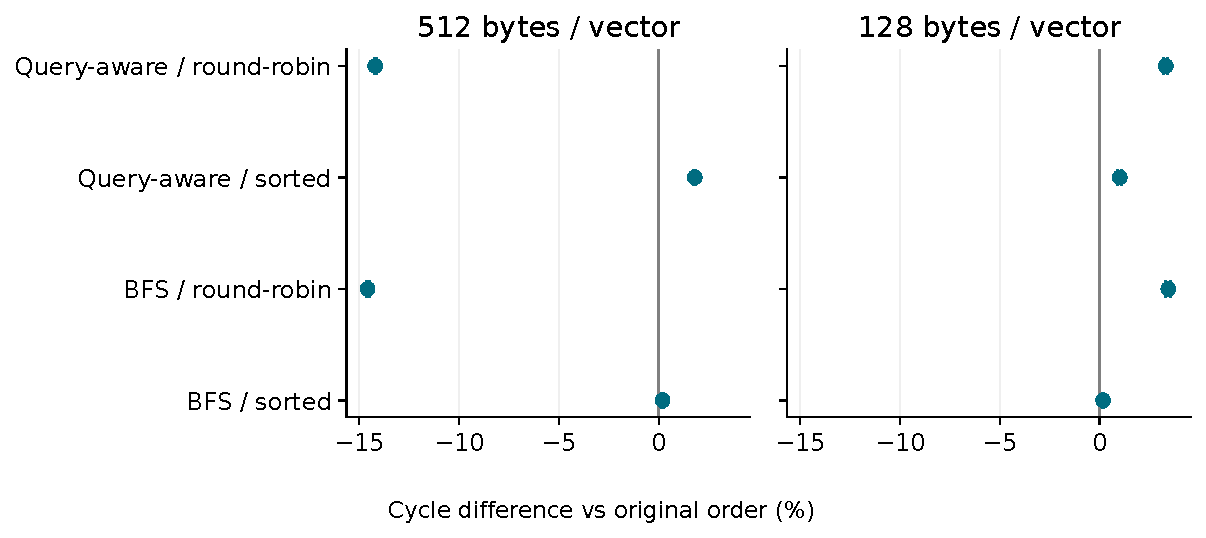
\includegraphics[width=0.92\textwidth]{generated/followup_schedules.pdf}
\caption{Available-request scheduling on the reference graph, ten paired splits. Points and bars show means and 95\% intervals. Both panels use the same scale; negative differences favour the schedule.}\label{fig:schedules}
\end{figure*}
